\documentclass{article}
\usepackage{mystyle}

\title{Notes on faster spherical harmonic expansion implementation}
\author{Scott Trinkle}
\date{Last edited: \today}
\begin{document}
\maketitle

\section{Introduction}
The two major steps in the pipeline for constructing a fiber orientation
distribution (FOD) from a cubic ROI of x-ray \uct data are (1) estimate the
local orientation at each voxel using structure tensor analysis, and (2) express
the distribution of these orientations using the spherical harmonics. Until now,
calculating the relevant spherical harmonic coefficients has been the major
computation bottleneck in this pipeline. This report details a new method for
calculating these coefficients using a spherical binning algorithm that improves
performance by nearly 100\% with no significant drop in accuracy.

\section{Previous implementation}
\subsection{From orientations to FOD}
The output of the structure tensor analysis algorithm for an ROI with a total of
$K$ elements is an array of $K$ vectors: \{$x_k, y_k, z_k$\}. With the current
implementation, these $K$ vectors are first converted into spherical
coordinates: \{$\theta_k, \phi_k$\} with $\theta \in [0, \pi]$ and
$\phi \in [0, 2\pi]$. The FOD is then represented as a sum of dirac delta
functions at these coordinates:
\begin{align}
  \label{eq:1}
  \text{FOD}(\theta, \phi) = \frac{1}{K}\sum_{k=1}^K \delta(\theta - \theta_k)\delta(\phi - \phi_k).
\end{align}

\subsection{Spherical harmonic representation}
The spherical harmonics are defined as
\begin{align}
  Y_l^m(\theta, \phi) = N_l^m P_l^m(\text{cos}\theta)e^{jm\phi},
\end{align}
where $N_l^m$ is a normalization coefficient, and $P_l^m$ are the
associated Legendre polynomials.

The SH form an orthonormal basis over $L_2(\mathbb{S}^2)$. Any
square integrable function $g(\theta, \phi) \in L_2(\mathbb{S}^2)$ can
be expressed as a linear combination of SH:
\begin{align}
  g(\theta, \phi) = \sum_{l=0}^{\infty}\sum_{m=-l}^l c_{lm}Y_l^m(\theta, \phi),
  \label{eq:SHexpand}
\end{align}
with coefficients $c_{lm}$ given by
\begin{align}
  c_{lm} = \int_{\mathbb{S}^2} g(\theta, \phi) \bar{Y}_l^m(\theta, \phi) \mathrm{d}\bm{\Omega},
  \label{eq:coeffs_0}
\end{align}
where the overbar denotes conjugation.

If we substitute Eqn. \ref{eq:1} into Eqn \ref{eq:coeffs_0}, then the sifting property of the Dirac
delta function can be used, and the integral reduces to:
\begin{align}
  c_{lm} = \frac{1}{K}\sum_{k=1}^K \bar{Y}_l^m(\theta_k, \phi_k).
  \label{eq:get_coeffs}
\end{align}
A SH approximation $\hat{\text{FOD}}(\theta, \phi)$ can then be determined to an arbitrary
band-limit $L_{max}$ using Eqn \ref{eq:SHexpand}.

Spherical harmonics are used extensively in the HARDI literature to represent
FODs. Generally, it is assumed that diffusion has even
symmetry, so odd-ordered SH components are assumed to be zero and
ignored. Furthermore, since the diffusion-weighted signal and ODF are both real
functions, their SH representations exhibit conjugate symmetry:
\begin{align}
  Y_{l}^m(\theta, \phi)_{real} \equiv
  \begin{cases}
    \sqrt{2}\text{Re}\left[Y_l^{|m|}(\theta, \phi)\right] & m < 0\\
    Y_l^0(\theta, \phi) & m = 0\\
    \sqrt{2}\text{Im}\left[Y_l^m(\theta, \phi)\right] & m > 0\\
  \end{cases}
  \label{eq:real_Y}
\end{align}

These simplifications hold true for the \uct FODs as well. In this work, we use a
band-limit of $L_{max} = 20$, for a total number of 231 even-ordered SH coefficients.

\subsection{Computational Expense}
With our current data, the \uct voxels are 1.2 $\upmu$m$^3$ isotropic, and the
MRI voxels are 150 $\upmu$m$^3$ isotropic. Accordingly, one MRI-voxel-sized ROI
includes a total of $K=125^3\approx 2$ million \uct voxels. The above
implementation thus requires each of the 231 even spherical harmonics up to
$L_{max}=20$ to be evaluated at 2 million points. Calculating all 231 of these
coefficients with this method for one ROI typically takes around 100 seconds on
the bigmem SIRAF nodes. There are approximately 500,000 voxels in the MRI data.
In order to create a corresponding \uct FOD for each of these voxels with this
method would thus take: 500,000 voxels $\times$ 100 seconds/voxel $\approx$
14,000 hours of computation time, not including the additional time needed
to estimate the orientations themselves.

\section{New implementation: spherical binning}
\subsection{From orientations to FOD}
The primary change comes in how the FOD is constructed from the orientation
vectors. Representing the FOD as a sum of $K\approx 2 \times 10^6$ delta
functions required each of the spherical harmonics to be evaluated at $K$
points. With the new method, the FOD is instead constructed as a histogram on
the sphere using $N$ approximately uniform sampling points as the bin centers.

The $N$ sampling points are chosen using a Fibonacci sampling
algorithm~\cite{Hannay2004}. The $K$ vectors are sorted into the corresponding
bins using a very fast nearest-neighbors search algorithm, implemented with a
\href{https://en.wikipedia.org/wiki/Ball_tree}{``ball tree''} nested data
structure in the
\href{http://scikit-learn.org/stable/modules/generated/sklearn.neighbors.NearestNeighbors.html#sklearn.neighbors.NearestNeighbors}{\texttt{scikit-learn}}
Python package.

This ``binned'' FOD can be written as a weighted sum of $N$ delta functions,
where $N \ll K$:
\begin{align}
  \label{eq:3}
  \text{FOD}_b = \frac{1}{K}\sum_{n=1}^N b_n \delta(\theta - \theta_n)\delta(\phi - \phi_n),
\end{align}
where $b_n$ is the bin count for the sampling point ($\theta_n, \phi_n$), and
$\sum_n b_n = K$.

\subsection{Spherical harmonic representation}
The calculation of the spherical harmonic coefficients proceeds in the same way. The
``binned'' FOD is substituted into Eqn \ref{eq:coeffs_0}, which results in:
\begin{align}
  c_{lm} = \frac{1}{K}\sum_{n=1}^N b_n \bar{Y}_l^m(\theta_n, \phi_n).
  \label{eq:4}
\end{align}
The same symmetries are exploited from Eqn \ref{eq:real_Y}.

\section{Results}

\begin{figure}[h]
  \centering
  \begin{subfigure}[n]{0.48\textwidth}
    \centering
    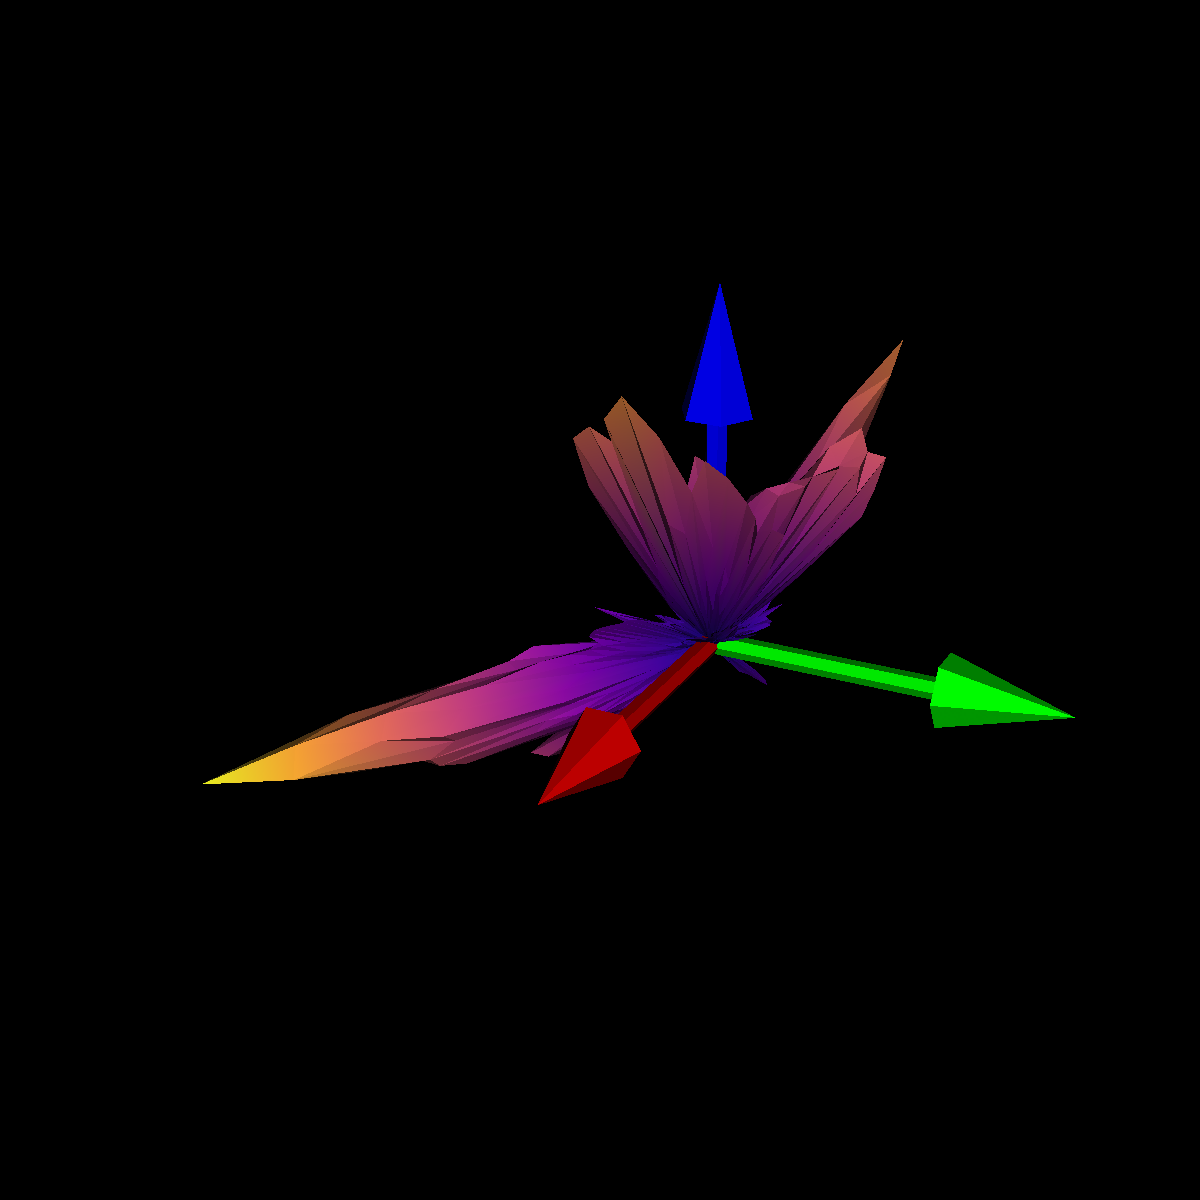
\includegraphics[width=0.8\linewidth]{../odf_comparison/raw_odf}
    \caption{Raw}
  \end{subfigure}
  \hspace{0.5em}
  \begin{subfigure}[n]{0.48\textwidth}
    \centering
    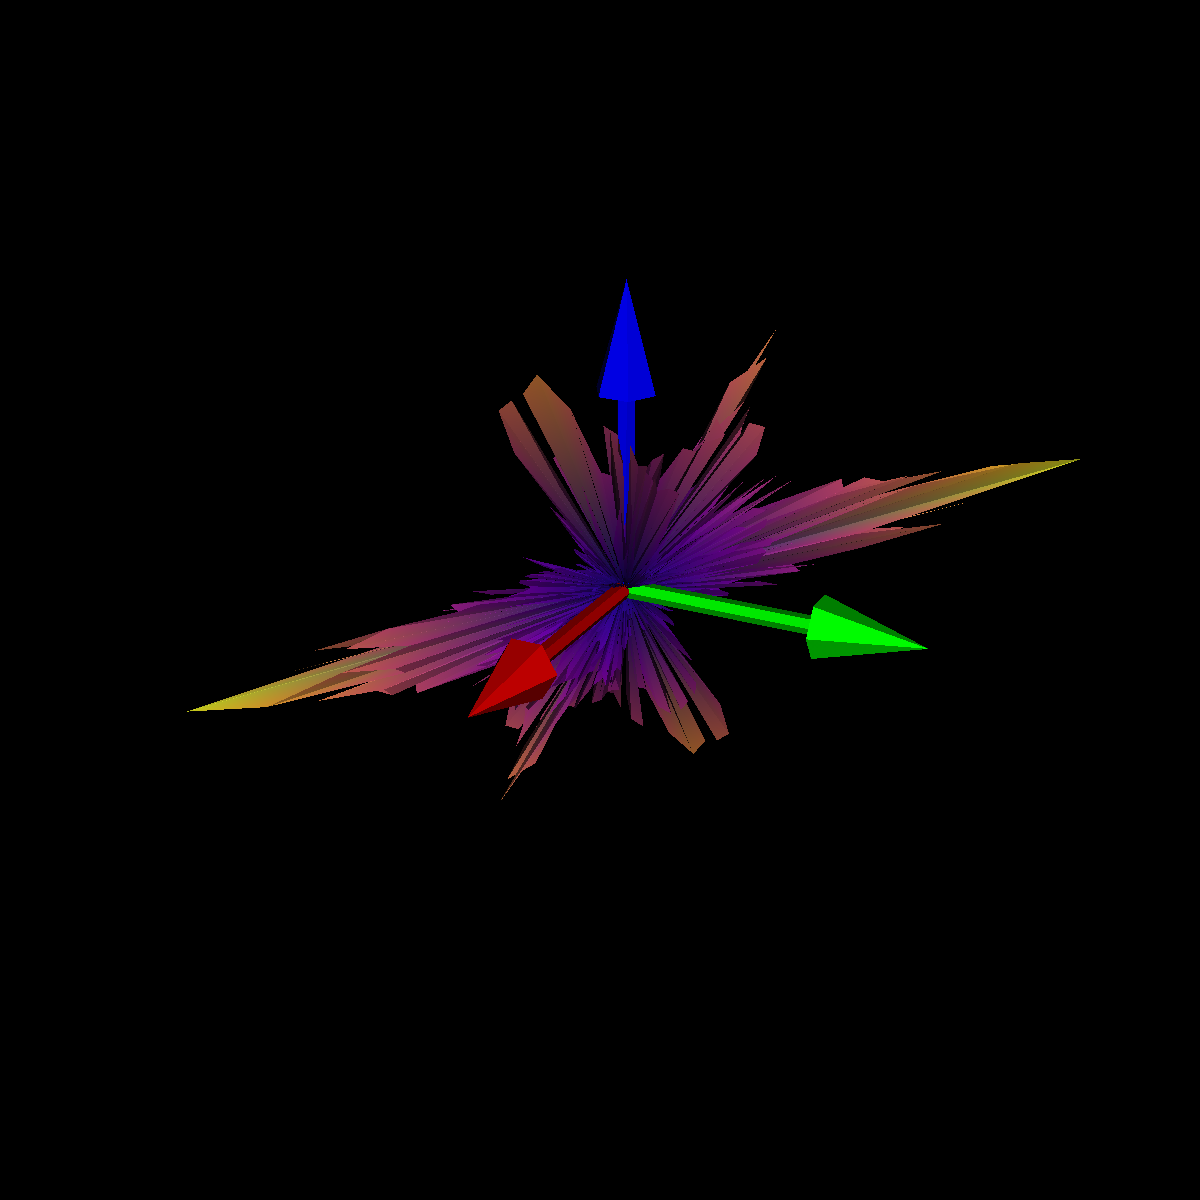
\includegraphics[width=0.8\linewidth]{../odf_comparison/raw_odf_even}
    \caption{``Forced-even''}
  \end{subfigure}
  \caption{The ``binned'' FOD}
  \label{fig:raw_fods}
\end{figure}

\bibliographystyle{ieeetr}
\bibliography{SH_speedup_notes}  
\end{document}